\documentclass[UTF8,12pt]{article}
\usepackage[utf8]{inputenc}
\usepackage[T1]{fontenc}
\usepackage{vmargin} % page format
\usepackage{soul}       % underline multiple lines
\usepackage{enumerate}
\usepackage{enumitem}
\usepackage{color}
\usepackage{amsmath}
\usepackage{multirow}
\usepackage{amssymb}
\usepackage{bbm}
\usepackage{graphicx}
\usepackage{subfig}
\usepackage{diagbox}
\usepackage{graphicx}
\usepackage{grffile}
\usepackage[pdfstartview=FitH,
CJKbookmarks=true,
bookmarksnumbered=true,
bookmarksopen=true,
colorlinks=true,                        
linkcolor=black]{hyperref}
\usepackage[numbers]{natbib}
\newcommand{\sinc}{\mathrm{sinc}}
\setpapersize{USletter}
\setmarginsrb{1 in}{1 in}{1 in}{0.5 in}{0pt}{0mm}{0pt}{0.5 in}
\pagestyle{empty}
\pagestyle{plain}
\setlength{\parskip}{1em}
\renewcommand{\baselinestretch}{1.5}
\usepackage{sectsty}% section font size
\usepackage{titlesec}% section spacing
\sectionfont{\fontsize{12}{0}\selectfont}
\subsectionfont{\fontsize{12}{0}\selectfont}
\titlespacing\section{0pt}{12pt plus 4pt minus 2pt}{0pt plus 2pt minus 2pt}
\titlespacing\subsection{0pt}{12pt plus 4pt minus 2pt}{0pt plus 2pt minus 2pt}
\titlespacing\subsubsection{0pt}{12pt plus 4pt minus 2pt}{0pt plus 2pt minus 2pt}

\title{Accomplishing Blind Source Separation using Independent Components Analysis (ICA)}
\date{2019\\ February}
\author{Yue WU\\ yw9998\\ sophywu@utexas.edu\\ CS 391L}
\begin{document}
	\maketitle
	\section{Introduction}
	This homework aims at using Independent Components Analysis (ICA) to accomplish Blind Source Separation. We will first mix n = 5 original signals into m = 8 mixed signals, and then reconstruct the original signals from the mixed signals by applying ICA.
	\section{Methods}
	We first mixed n = 5 original signals stored in matrix U into m = 8 mixed signals stored in matrix X by multiplying the matrix U with matrix $A\in \Re ^{m*n}$ (Equation \ref{eq:mixing}). Values in A were chosen randomly and were ranged between 0 and 1. A indicates how much each original signal is contributing to each mixed signal.
	\begin{equation}
	\label{eq:mixing}
	X = AU
	\end{equation}
	
	Then we started to reconstruct the original signals. We first initialized a random matrix $W\in \Re ^{n*m}$. Values in W ranges between 0 and 0.1. Multiplying W with X gave us reconstructed signals stored in matrix Y (Equation \ref{eq:reconstruct}). The matrix Y is of the same size as the matrix U.
	\begin{equation}
	\label{eq:reconstruct}
	Y = WX
	\end{equation}
	
	However, after the very first step the matrix Y was still very different from the matrix U. Therefore we need to apply the algorithm to keep updating the matrix W until the matrix Y becomes similar to the matrix U. The algorithm consists of the following two equations. Equation \ref{eq:gradient}is used to calculate gradients of every element in the matrix Y and Equation \ref{eq:updatevalue}is used to calculate the amount of update, where $\eta$ represents the learning rate and t represents the number of values in each signal. We divided t here to prevent overflow. We will discuss how the choosing of $\eta$ can affect our results in the following section. We then update the matrix W using Equation \ref{eq:update}. After that, we checked the convergence condition by calculating the differences between the current recovered signal and the previous recovered signal (Equation \ref{eq:covcheck}). We found out the maximum value in the matrix C and compared it with a "judging" value we set at the beginning of the iterations. When the maximum value in the matrix C is smaller than the "judging value", we consider the iteration has converged and completed. The last step is noting down the number of iterations we took to arrive at the "judging value".
	\begin{equation}
	\label{eq:gradient}
	z_{i,j} = g(y_{i,j}) = \frac{1}{1+e^{-y_{i,j}}}
	\end{equation}
	\begin{equation}
	\label{eq:updatevalue}
	\Delta W = \eta (I+\frac{(1-2Z)Y^{T}}{t})W
	\end{equation}
	\begin{equation}
	\label{eq:update}
	W = W+\Delta W
	\end{equation}
	\begin{equation}
	\label{eq:covcheck}
	C = abs(\Delta W*X)
	\end{equation}
	
	\section{Results}
	We first tested our algorithm using the test set (Figure \ref{fig:test}). The top three lines are the recovered signals; the three lines in the middle are the mixed signals; the three lines shown at the bottom are the original signals. By setting the learning rate $\eta$ to be 0.01, we nearly fully recovered the signals although the sequence was different from the sequence at the beginning.
	\begin{figure}[!ht]
	\centering
	\subfloat[]{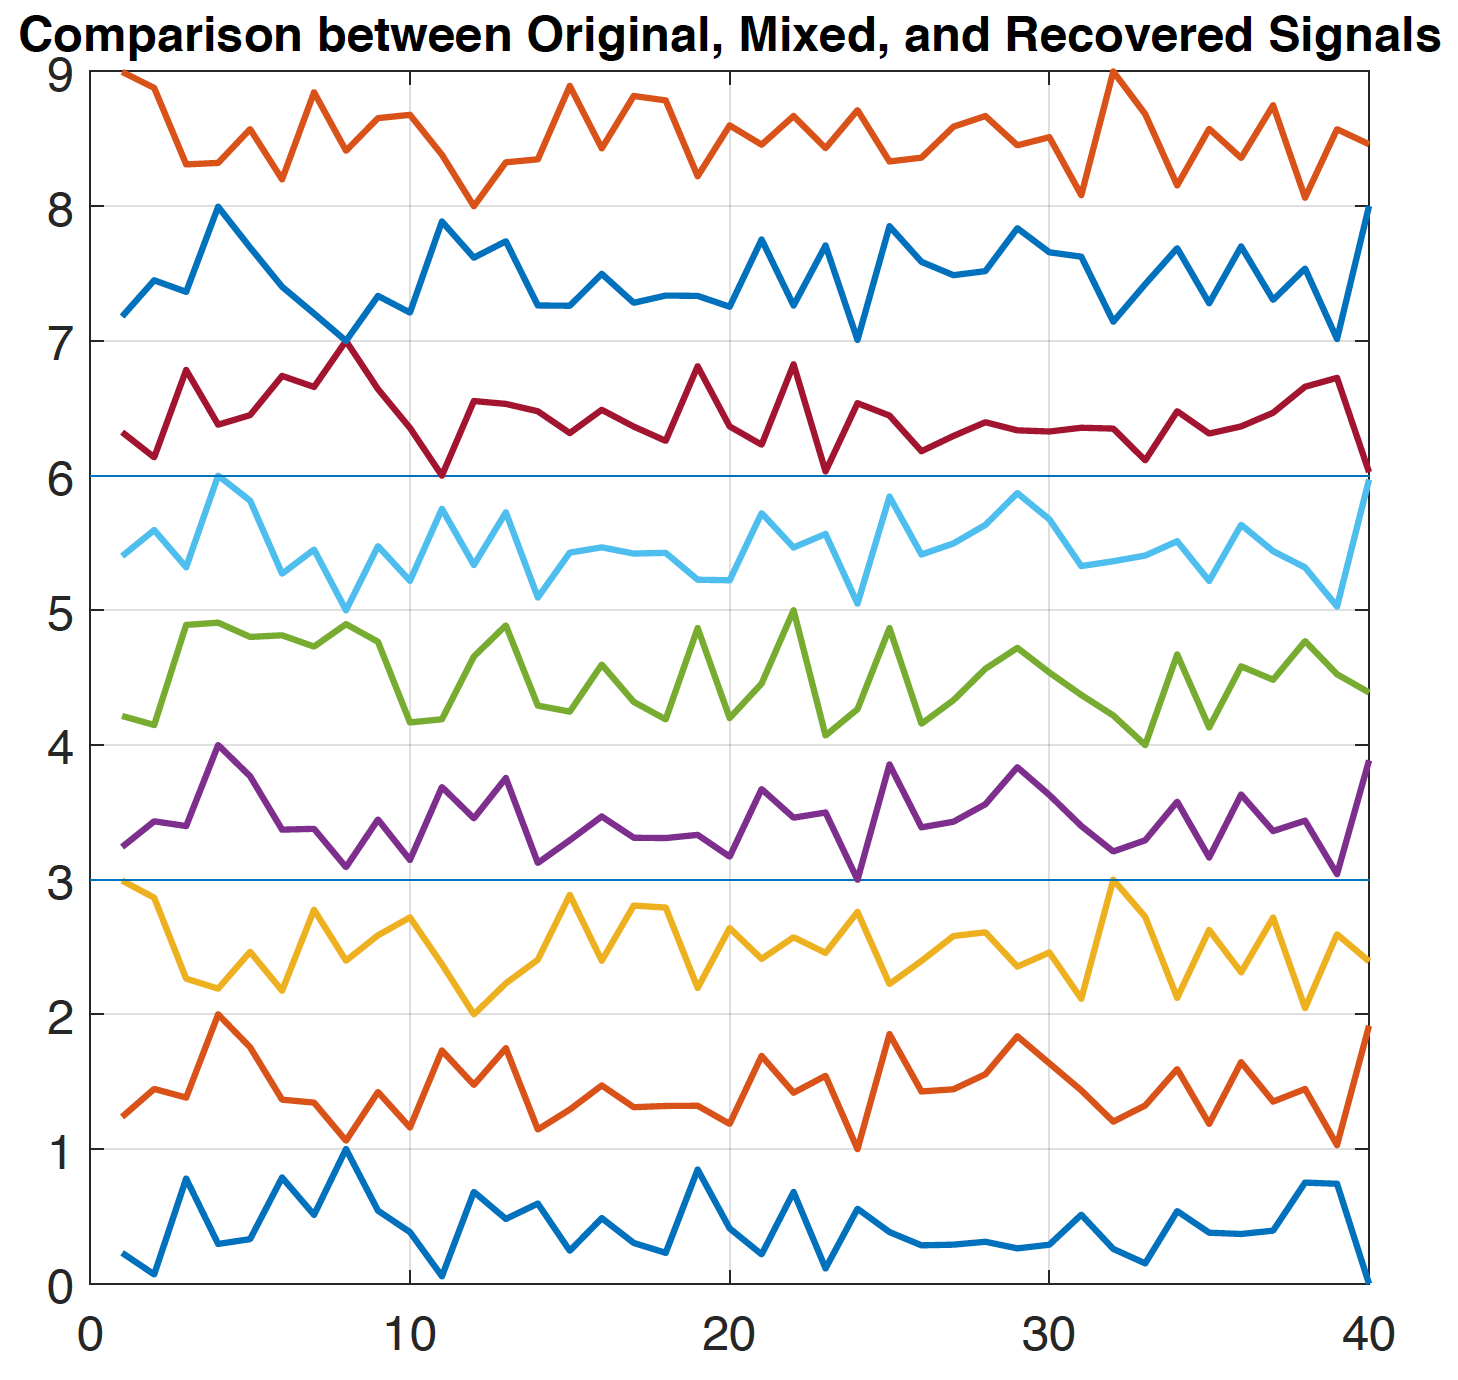
\includegraphics[width=0.8\linewidth]{figures/1.png}}
	\caption{\label{fig:test}Results from the test set. The top three lines are the recovered signals; the three lines in the middle are the mixed signals; the three lines shown at the bottom are the original signals.}
	\end{figure}	

	We then mixed all five original signals into eight mixed signals and reconstructed the original signals using the algorithm. We tested for three $\eta$s: 0.1, 0.01, and 0.001. We recorded the variation of the maximum value in matrix C with iterations. When the maximum value started to change slowly and finally reach the "judging value", the iterations stopped, and we considered the process completed. Since the restored signals might be in a different sequence as the original signals, we compare the shape of each restored signals with the shape of each original signals by calculating the correlation coefficients. Since the "judging values" we set are typically very small, when the restored signals matched with the original signals, the correlation coefficients can reach 0.9999. After matching the signals, we normalized the restored signals so that their values still ranged between -1 and 1. The results are shown in Figure \ref{fig:sound1}, Figure \ref{fig:sound2} and Figure \ref{fig:sound3} for three distinct $\eta$s.
	\begin{figure}[!ht]
		\centering
		\subfloat[][]{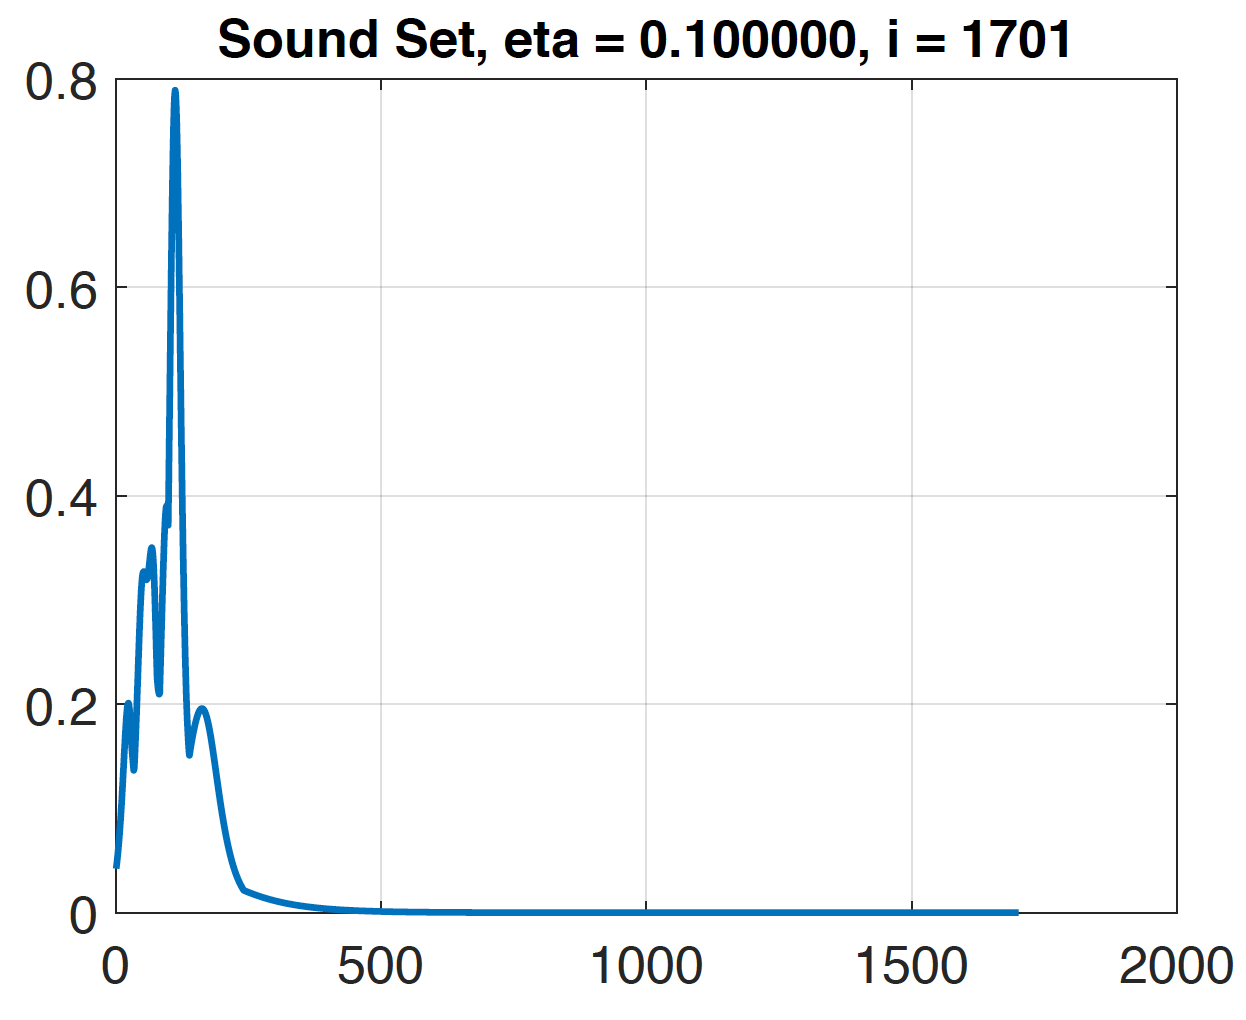
\includegraphics[width=.4\textwidth]{figures/2.png}}\quad
		\subfloat[][]{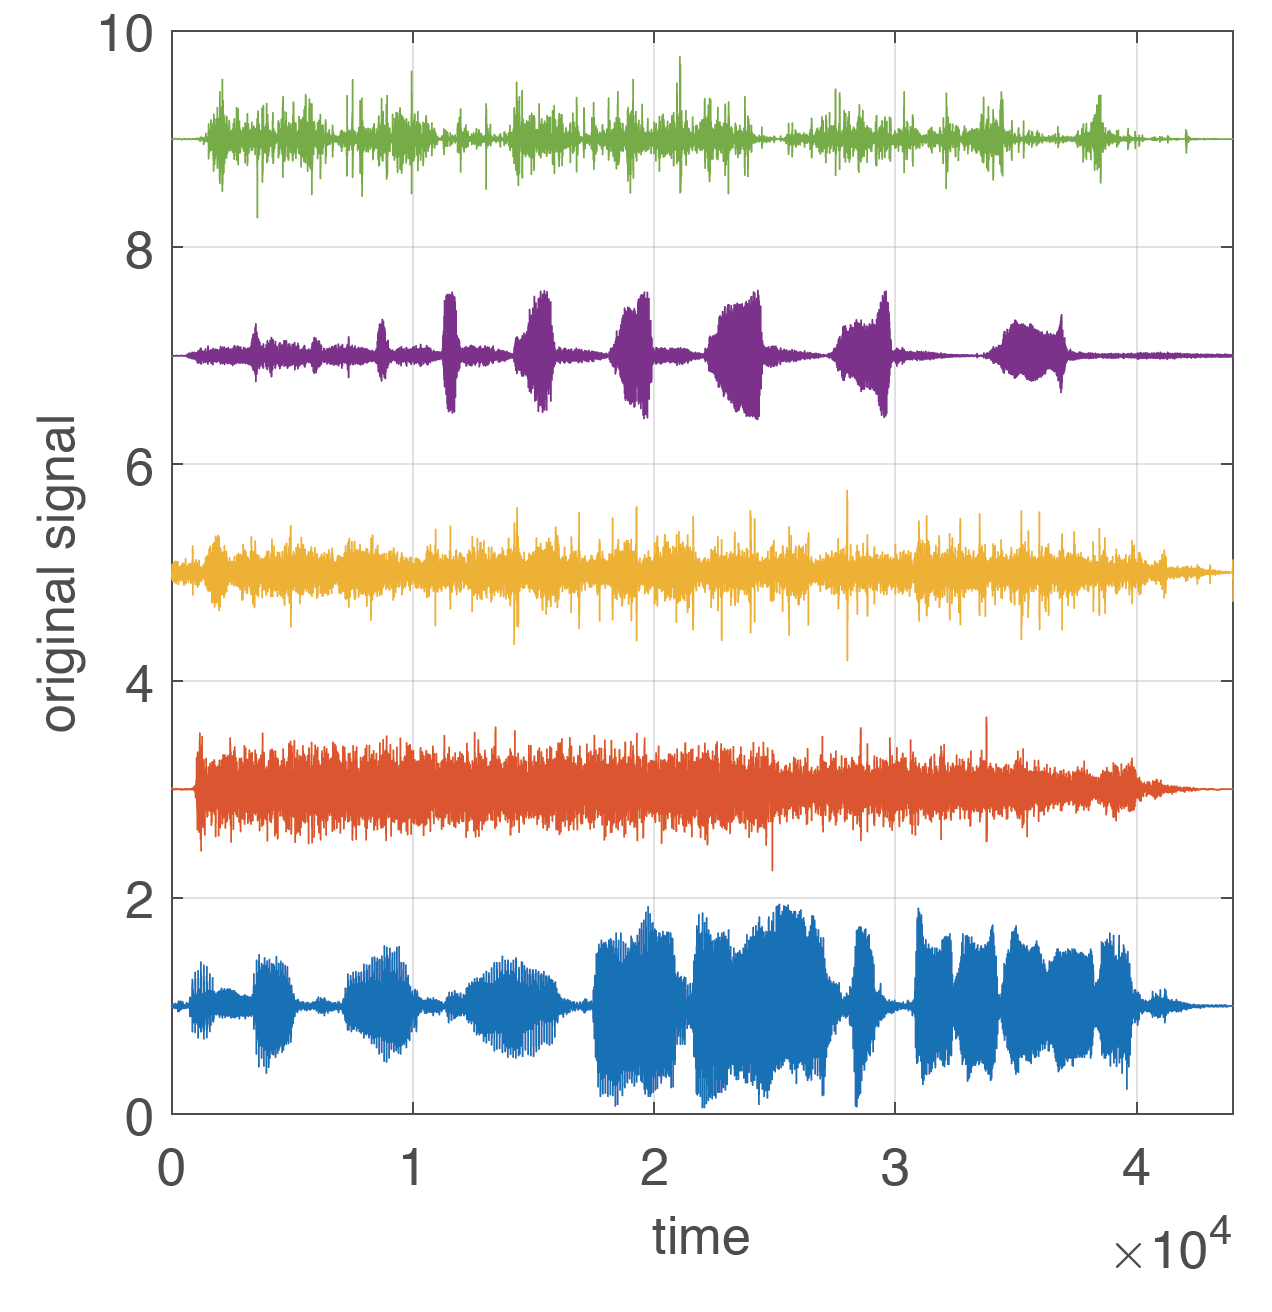
\includegraphics[width=.4\textwidth]{figures/3.png}}\\
		\subfloat[][]{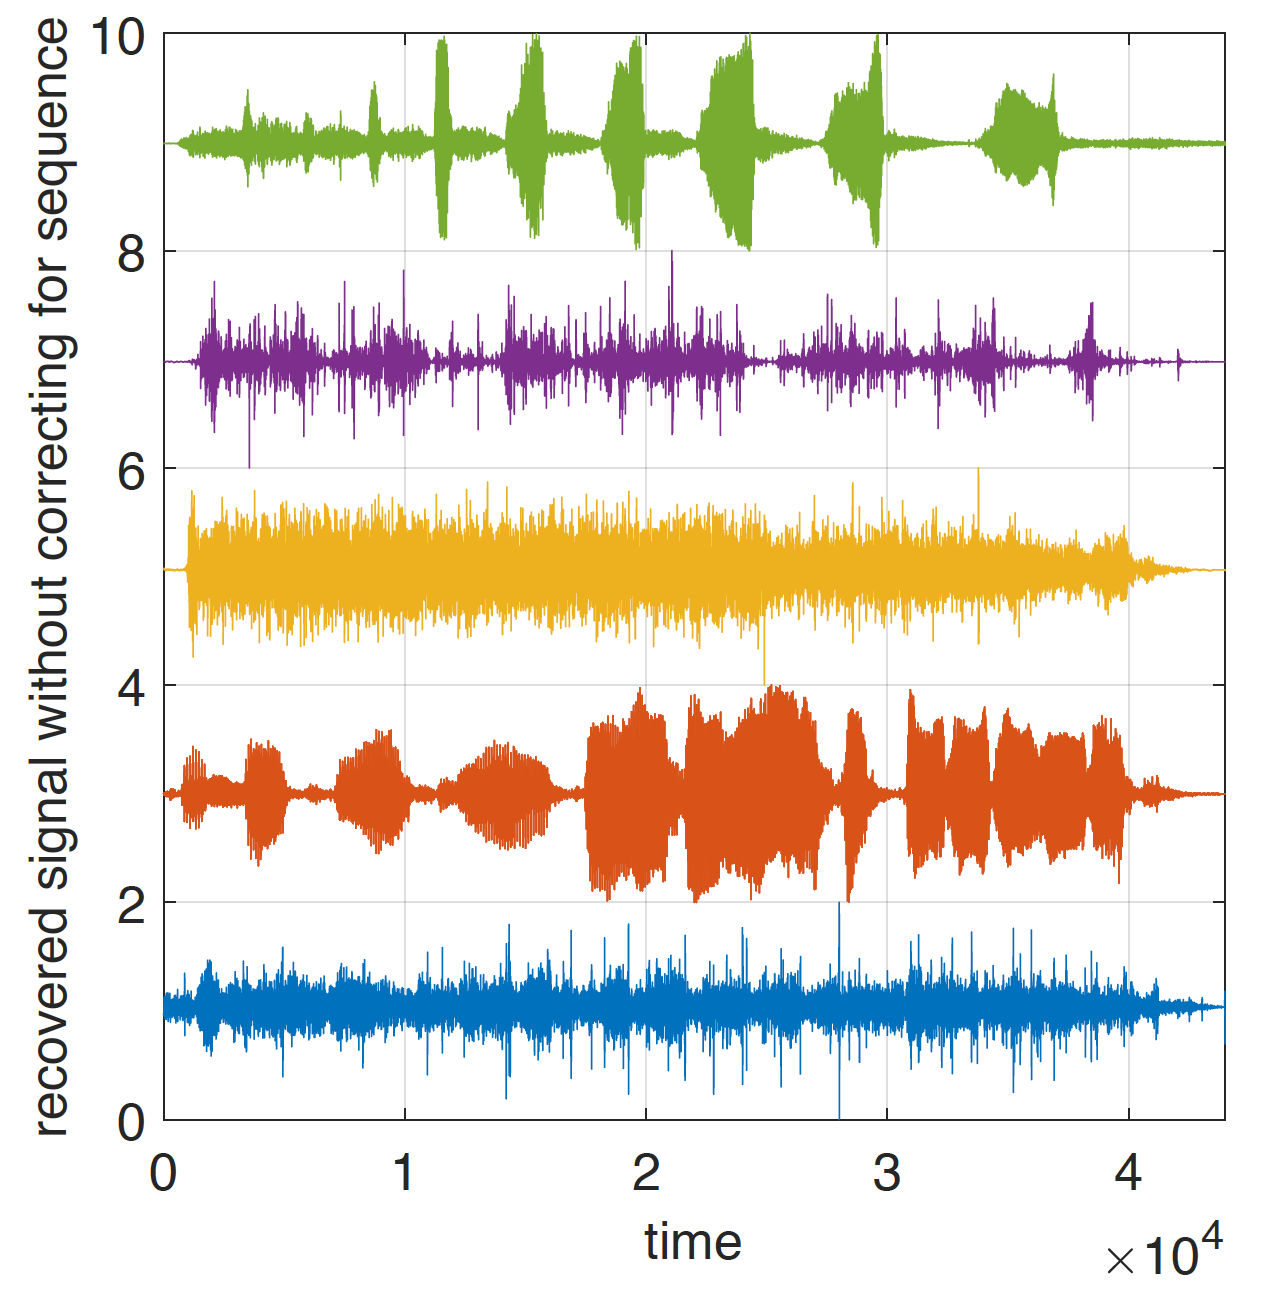
\includegraphics[width=.4\textwidth]{figures/4.png}}\quad
		\subfloat[][]{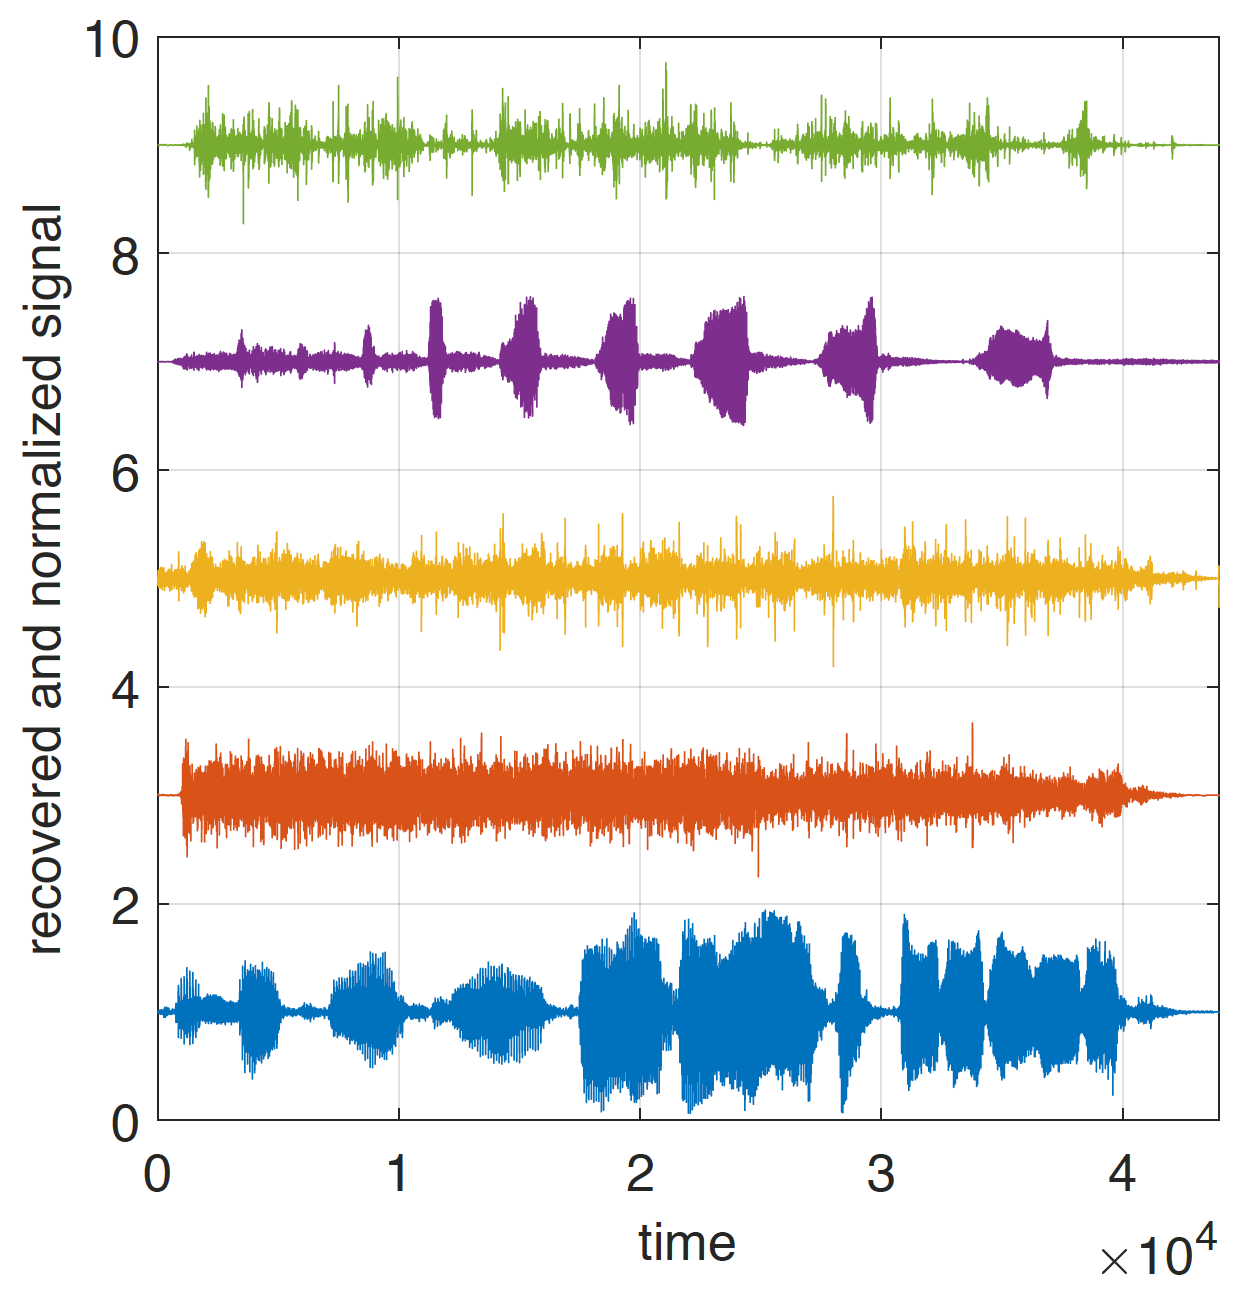
\includegraphics[width=.4\textwidth]{figures/5.png}}
		\caption{\label{fig:sound1} This figure shows the situation where the learning rate is 0.1. (a) Variance of the difference between the current recovered signal and the previous recovered signal with iterations (b) Original signals (c) Restored signals before correcting for sequence and normalization (d) Restored images}
	\end{figure}
	\begin{figure}[!ht]
		\centering
		\subfloat[][]{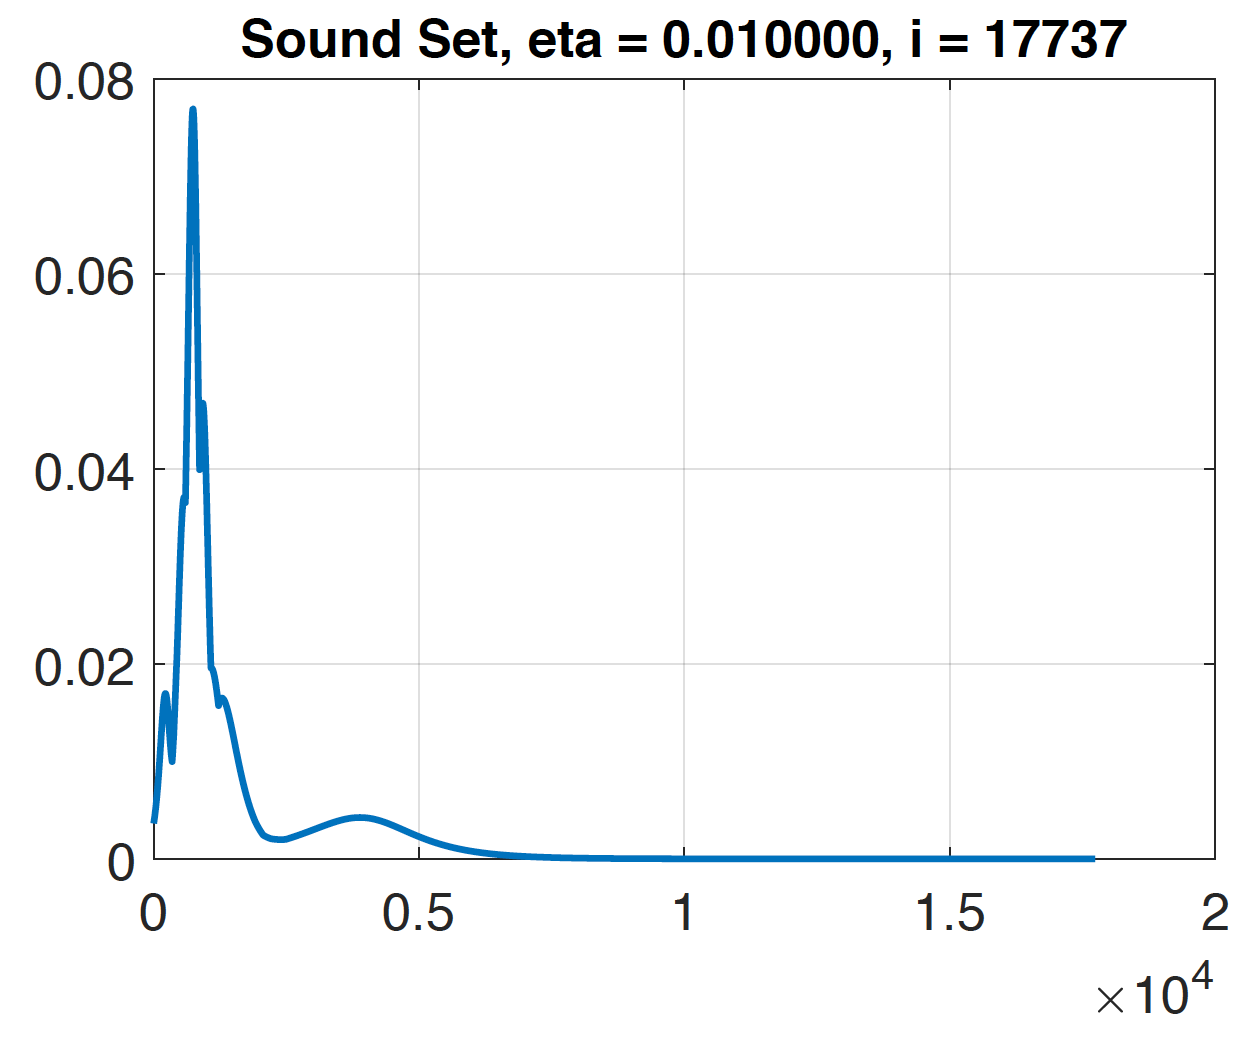
\includegraphics[width=.4\textwidth]{figures/6.png}}\quad
		\subfloat[][]{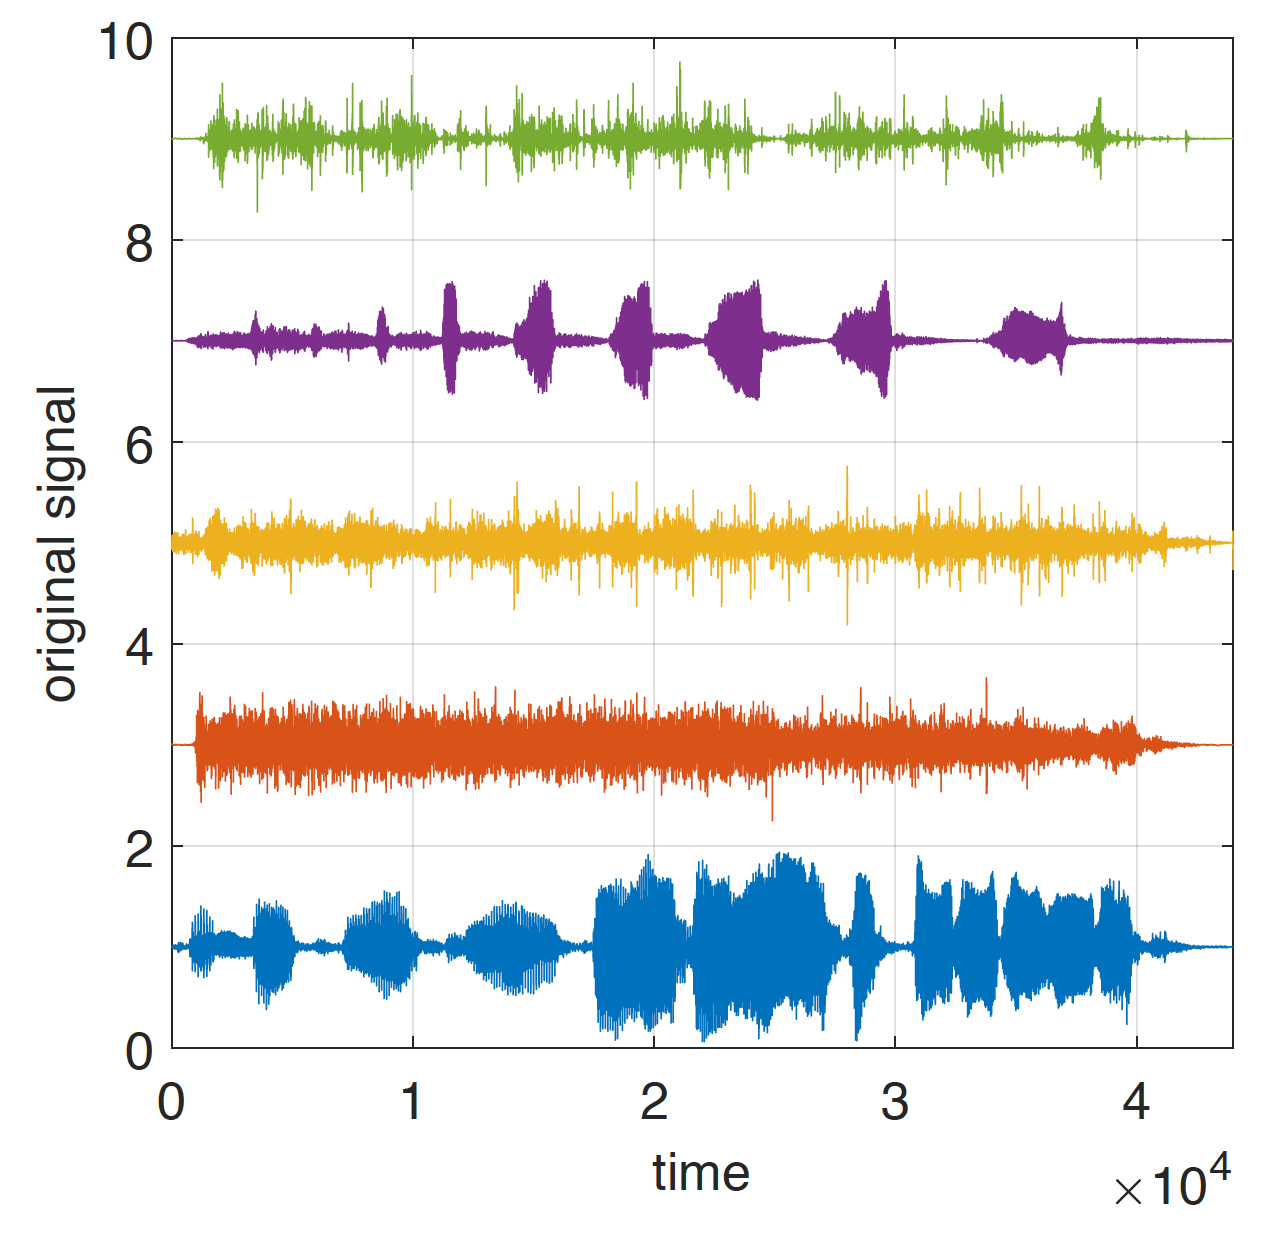
\includegraphics[width=.4\textwidth]{figures/7.png}}\\
		\subfloat[][]{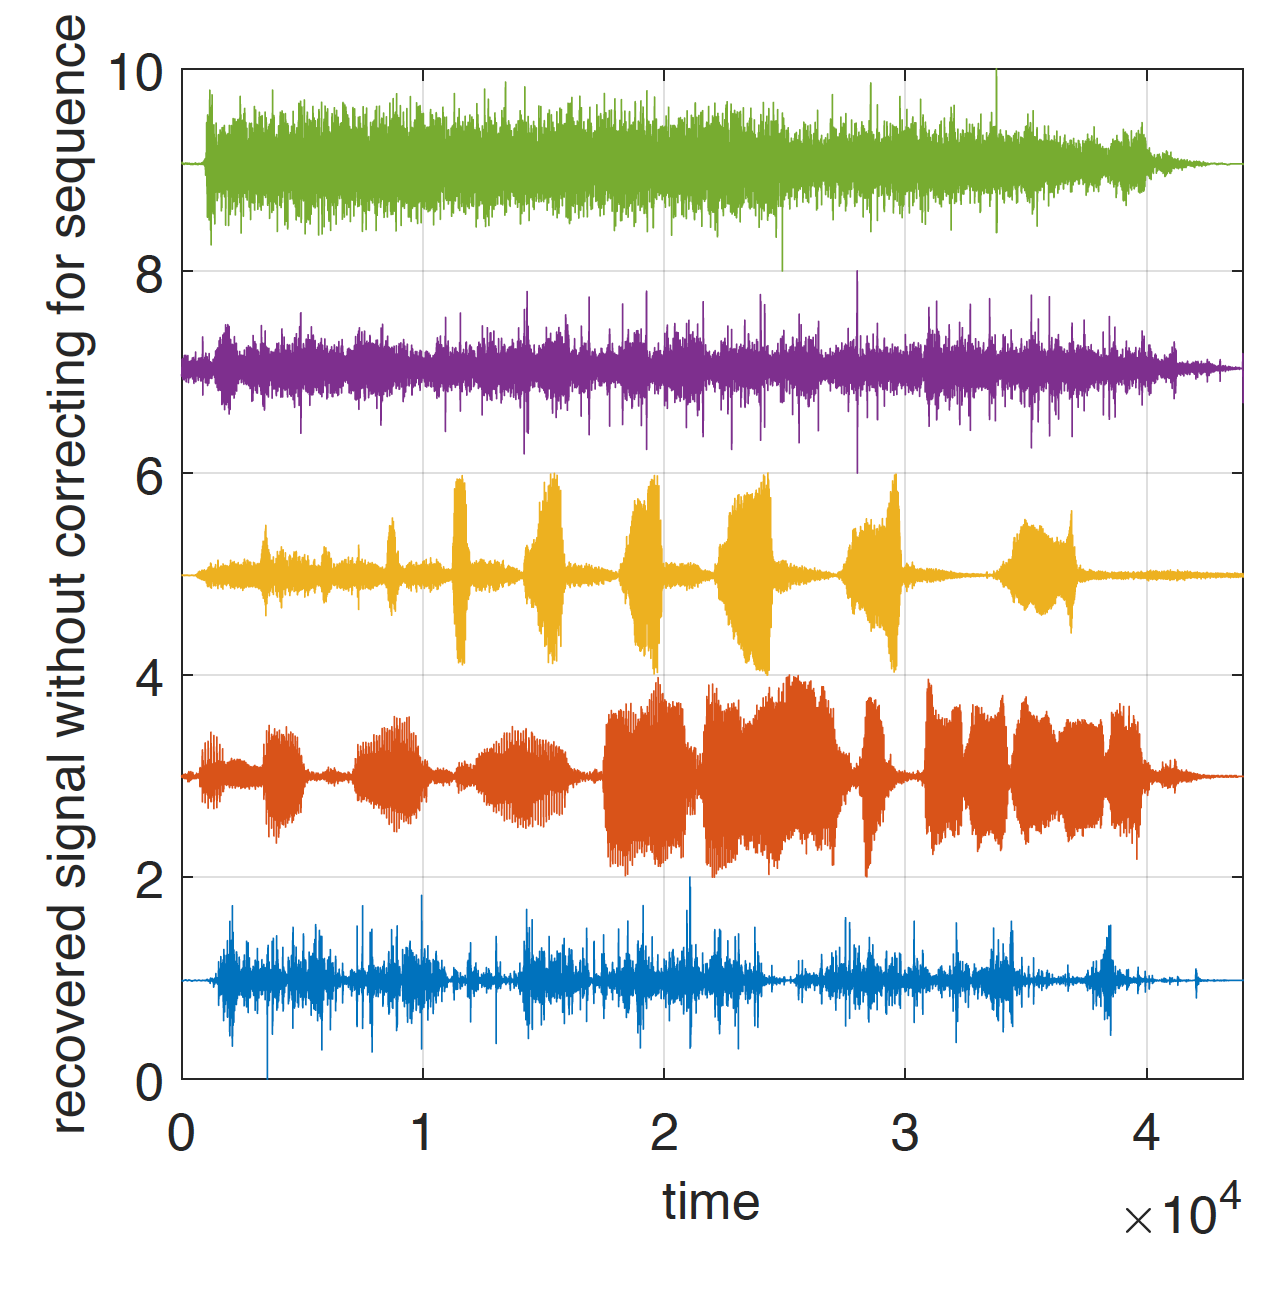
\includegraphics[width=.4\textwidth]{figures/8.png}}\quad
		\subfloat[][]{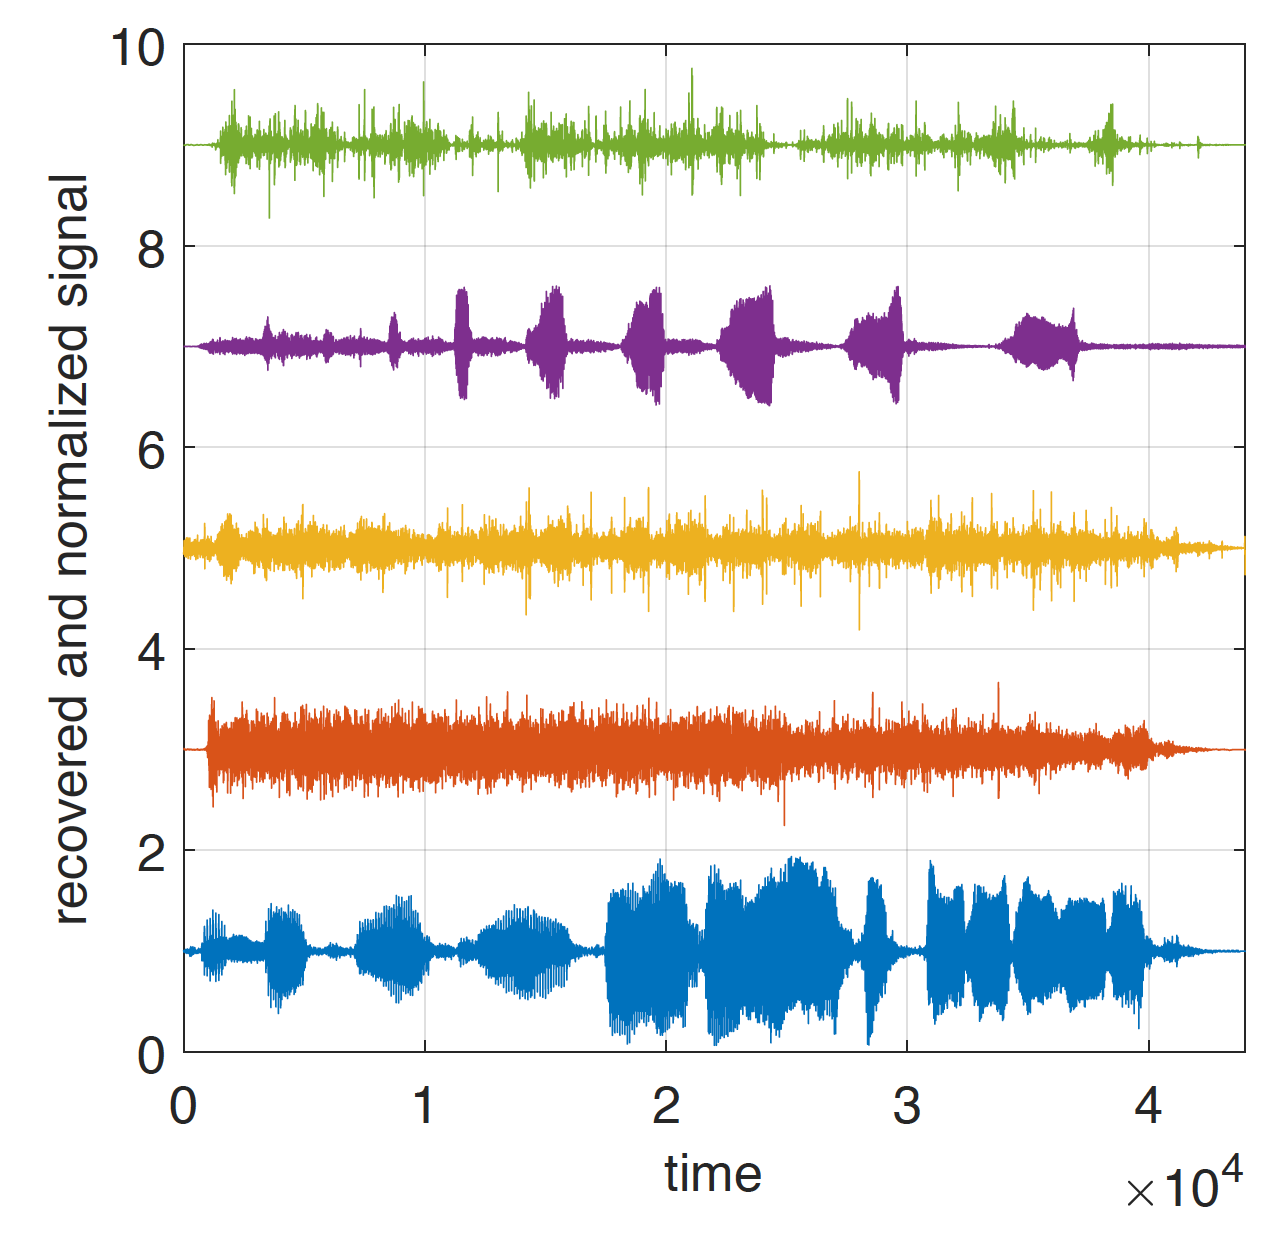
\includegraphics[width=.4\textwidth]{figures/9.png}}
		\caption{\label{fig:sound2}This figure shows the situation where the learning rate is 0.01. (a) Variance of the difference between the current recovered signal and the previous recovered signal with iterations (b) Original signals (c) Restored signals before correcting for sequence and normalization (d) Restored images}
	\end{figure}
	\begin{figure}[!ht]
		\centering
		\subfloat[][]{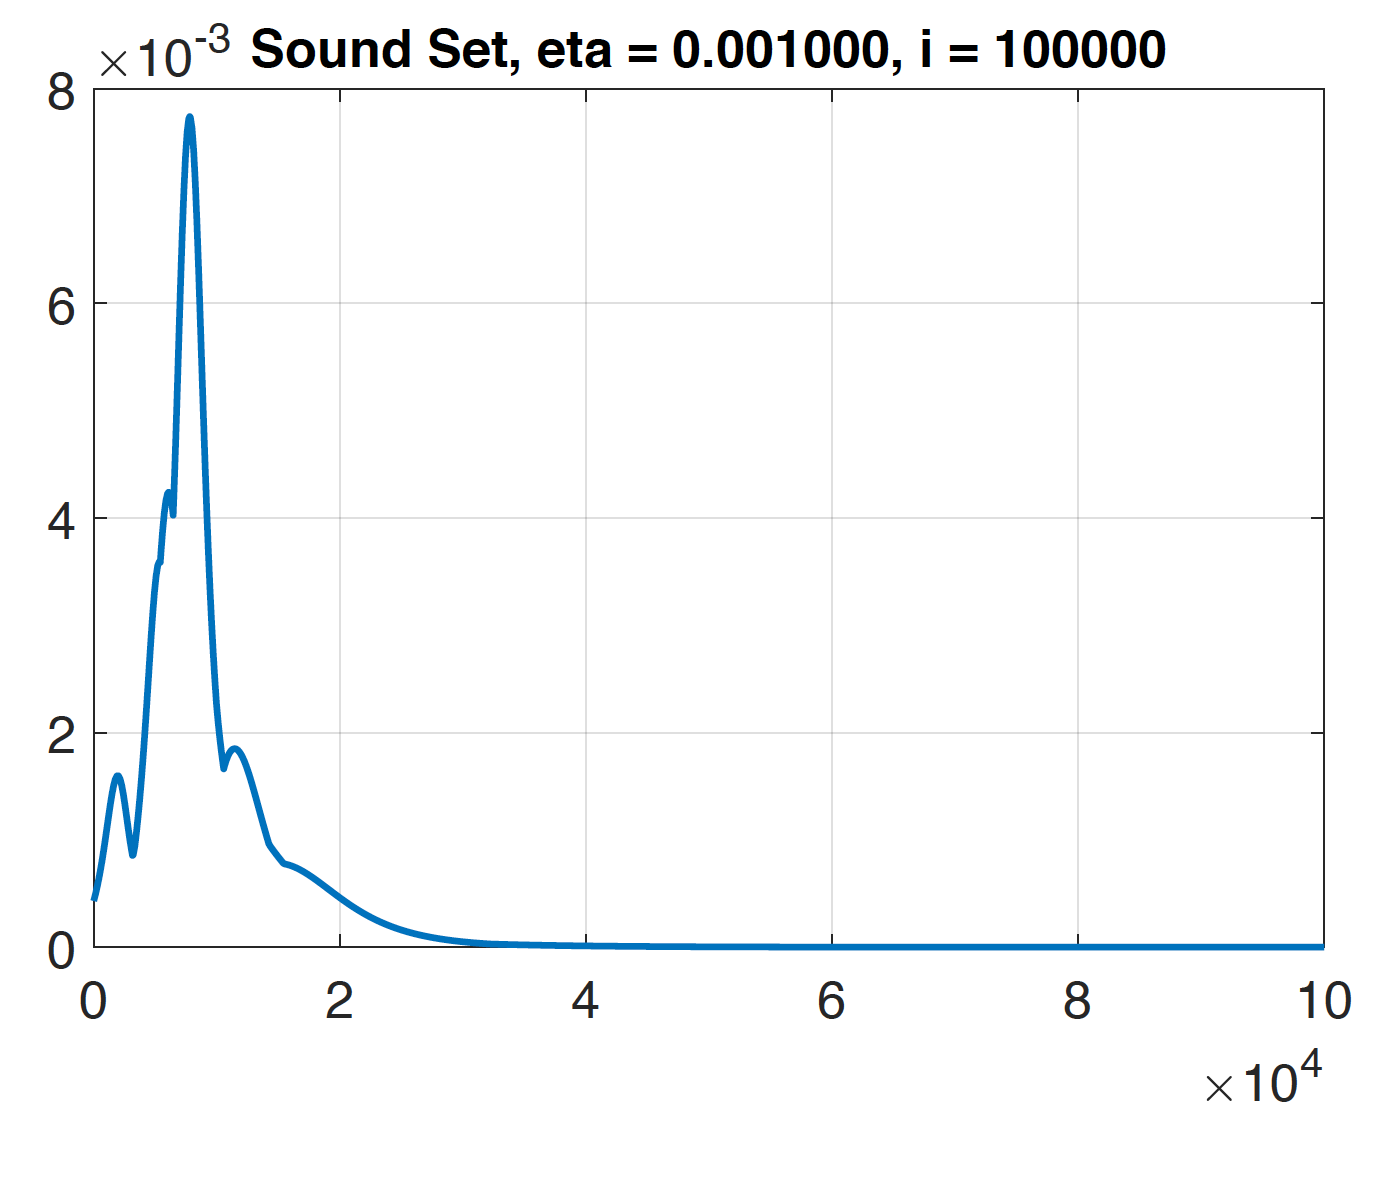
\includegraphics[width=.4\textwidth]{figures/10.png}}\quad
		\subfloat[][]{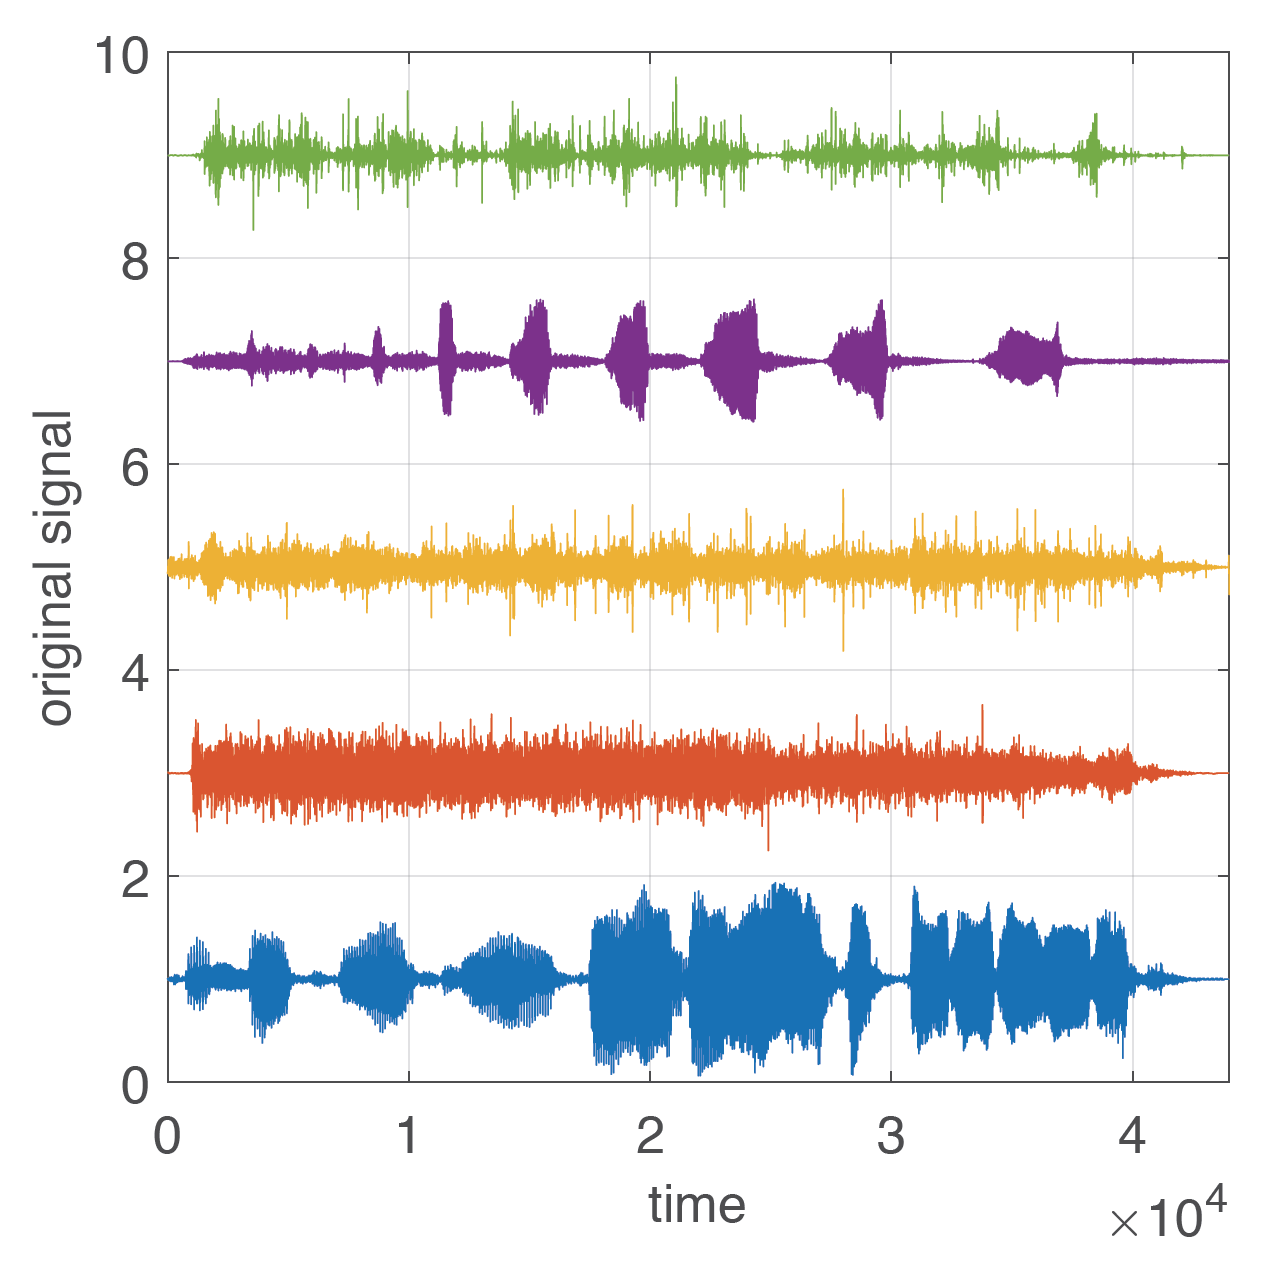
\includegraphics[width=.4\textwidth]{figures/11.png}}\\
		\subfloat[][]{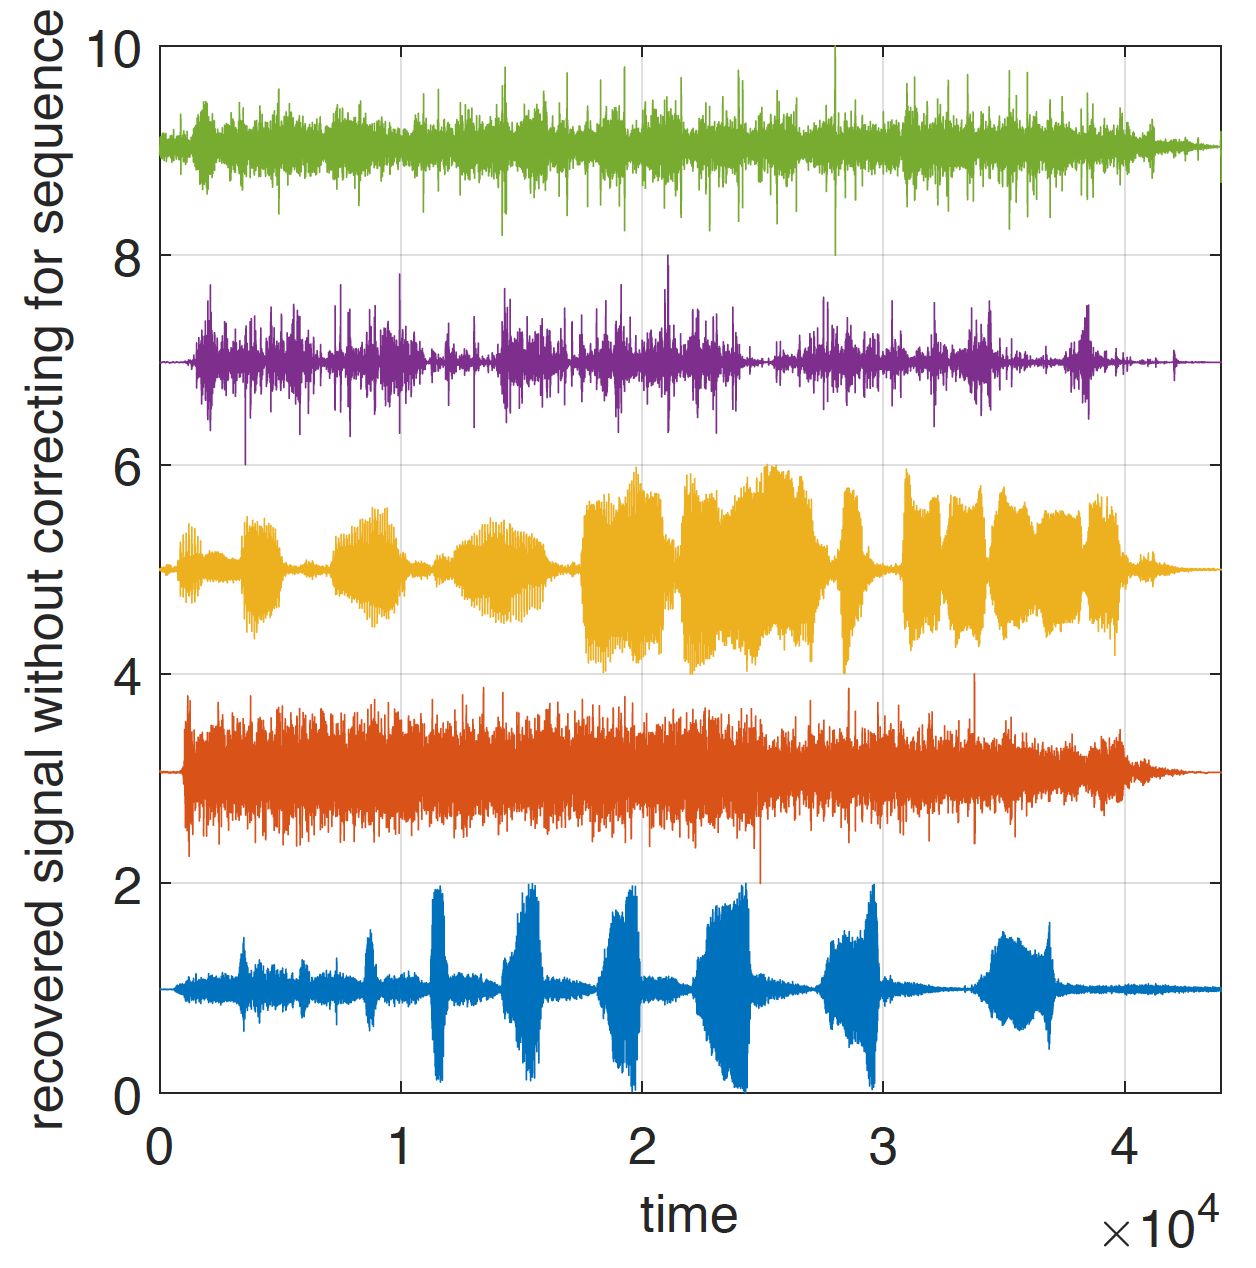
\includegraphics[width=.4\textwidth]{figures/12.png}}\quad
		\subfloat[][]{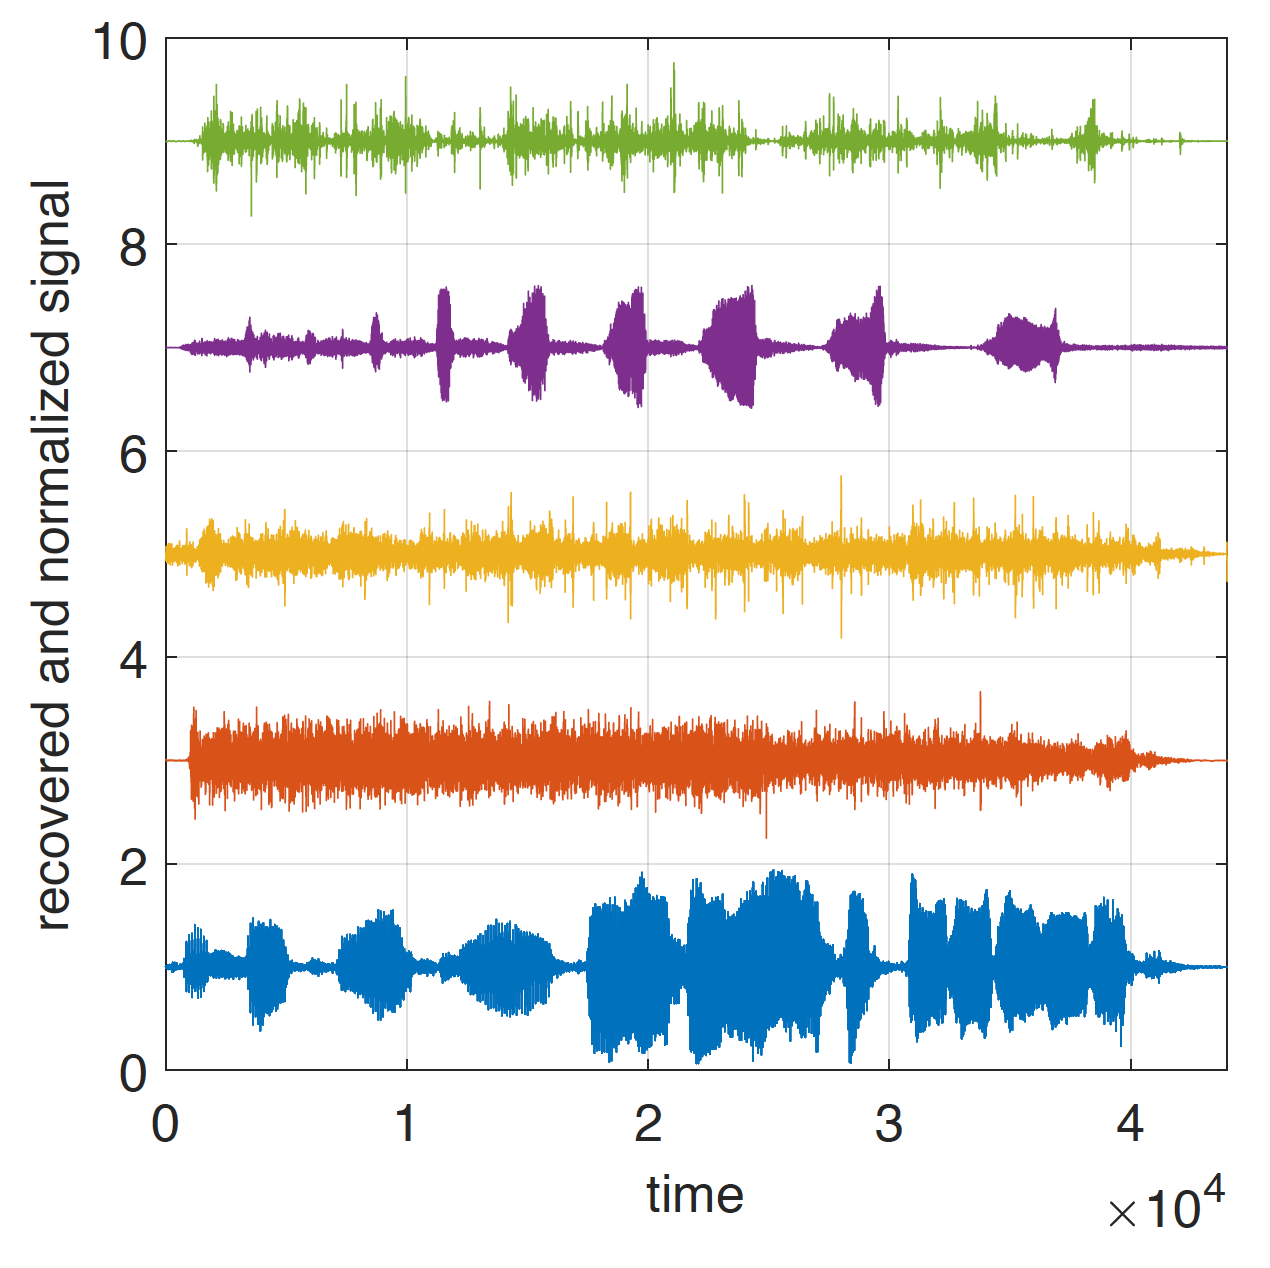
\includegraphics[width=.4\textwidth]{figures/13.png}}
		\caption{\label{fig:sound3}This figure shows the situation where the learning rate is 0.001. (a) Variance of the difference between the current recovered signal and the previous recovered signal with iterations (b) Original signals (c) Restored signals before correcting for sequence and normalization (d) Restored images}
	\end{figure}
	\section{Conclusion}
	We have mentioned in the previous section that when the restored signals matched the original signals, the correlation coefficients can reach 0.9999. This indicates that the restored signals were very similar or almost the same as the original signals. This remains true for all three $\eta$s.
	
	Convergence of Gradient Descent varied with regard to learning rate $\eta$ as is shown in Figure (a) in Figure \ref{fig:sound1}, Figure \ref{fig:sound2} and Figure \ref{fig:sound3}. We set the "judging value" to be $10^{-9}$, which means that when the maximum value in the matrix C is lower than this value, or in other words, when the difference between the current recovered signal and the previous recovered signal is smaller than this value, the iterations would stop, and we considered that we had reached convergence. When $\eta = 0.1$,  we reached convergence after only 1701 iterations. When $\eta = 0.01$,  we reached convergence after 17737 iterations. When $\eta = 0.01$,  we did not reach the "judging value" after 100000 iterations. The final difference that we arrived at after 100000 iterations was only  $10^{-8}$. To conclude, as the learning rate $\eta$ decreases, it took longer to reach convergence (Table \ref{table:convergence}).
	\begin{table}[]
		\begin{tabular}{l|l|l}
			\hline
			$\eta$ & Maximum value in the matrix C & \# of iterations \\\hline
			0.1    & $10^{-9}$                     & 1701             \\
			0.01   & $10^{-9}$                     & 17737            \\
			0.001  & $10^{-8}$                     & 100000           \\\hline
		\end{tabular}
		\caption{\label{table:convergence}The optimal number of eigenvalues used for different numbers of training samples as well as the corresponding accuracy.}
	\end{table}
\end{document}